\chapter{Background}
    This chapter discusses the required background information needed for a better understanding of the proposed work. In the first section explains the overall architecture of ITS and their components. The second section discusses the current state-of-the-art techniques used to perform ITS simulation. At last, an overview of the tools used to build the framework is given.
\section{Intelligent Transportation System}
\begin{figure}[h!]
    \centering
    
    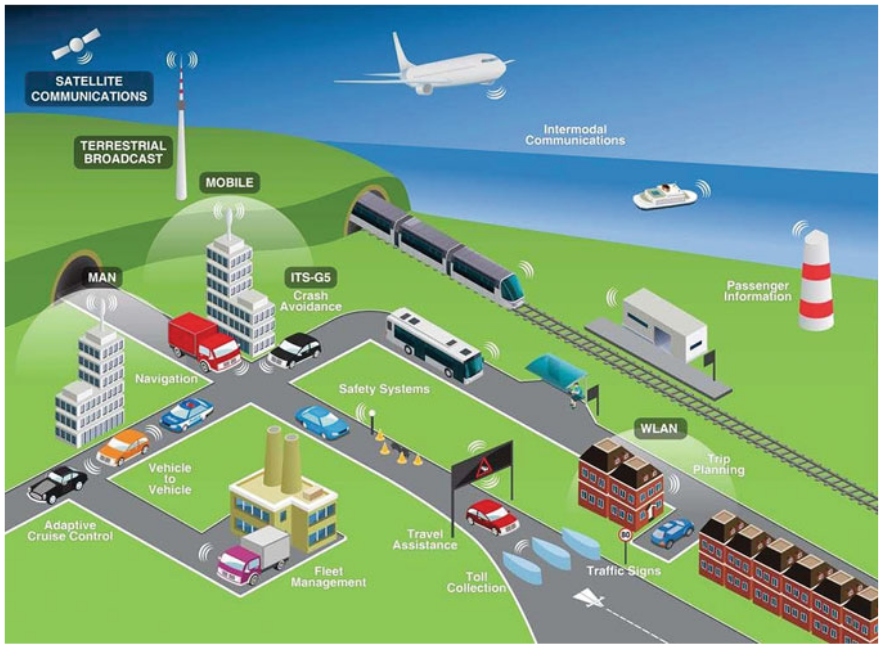
\includegraphics[width=10cm]{Framework/Images/CITS.png}.
    \caption{C-ITS Environment \cite{etsiDENM}}
    \label{cits}
\end{figure}

The Intelligent Transportation Systems (ITS) comprises of different applications that improve the safety, security and efficiency of transportation and provide a better driving experience. ITS achieves this by gathering necessary data from the sensors or devices placed in the infrastructure or vehicles. Initially, ITS only provided intelligence to vehicles  and roadside infrastructure, it was not able to share information between them and make them cooperate to regulate the traffic. 
The European Commission introduced the Cooperative Intelligent Transportation System as a new category of ITS \cite{alam_ferreira_fonseca_2016}. In which drivers, vehicles, passengers or road operators can directly interact with each other or with the surrounding infrastructure and figure \ref{cits} illustrates a typical CITS environment. CITS takes advantage of the communication and cooperation between different actors and effectively regulate the traffic flow by exchanging information about traffic jams, congestion, accidents. 

\subsection{Architecture}
Intelligent Transportation System consists of four sub-systems or stations \cite{etsi}, that helps transportation infrastructure to gain intelligence and real-world information . All the Sub-Systems are made up of ITS Station (ITS-S), it may contain a single ITS-S or network of ITS-S. 

\subsubsection{ITS Station Reference Architecture}
The ITS Station is the base component upon which a sub-system is built and its reference architecture helps to understand the functionality of ITS Station. Its architecture follows the principles of the OSI model\cite{OSI} for the layered communication protocol, and it is extended to include different ITS applications. In the figure \ref{ci88ts-s},

\begin{itemize}
\item Access layer is responsible for the functionality of Physical and Data Link layers
\item Network and Transport layer is responsible for the functionality of  Network and Transport layers
\item Facilities layer is responsible for the functionality of Session, Presentation and Application layers
\item Application layer
\item Management layer is responsible for managing the communication with the ITS Station
\item Security layer is responsible for providing security services to ITS Station and it is also considered as a part of  management entity.
\end{itemize}

\begin{figure}[h!]
    \centering
    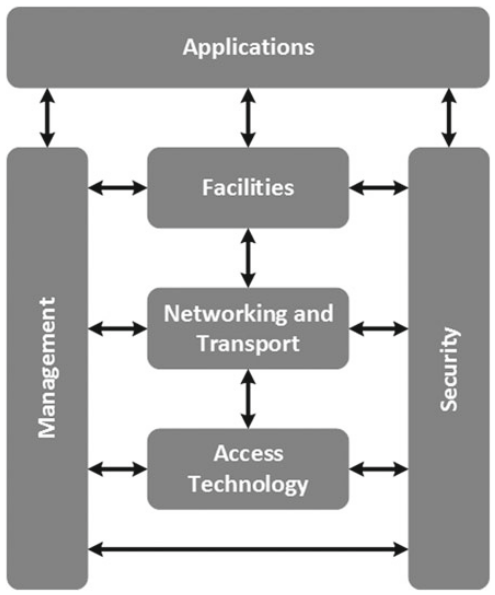
\includegraphics[scale=0.40]{Framework/Images/ITS-SRefArc.png}.
    \caption{ITS Station Reference Architecture }
    \label{ci88ts-s}
\end{figure}

\subsubsection{Functional Components of ITS Station}
 Based on their functionality, ITS Station can be divided into four sub-clauses \cite{etsi}
\begin{itemize}
    \item \textbf{Host :} It helps to run the ITS application
    \item \textbf{Gateway :} It helps to connect a ITS Station with the external propriety network. Facilities layer helps to connect different protocols.
    \item \textbf{Router :} It helps to connect one ITS Station with another. Network and transport layer helps to connect different ITS-S.
    \item \textbf{Border Router :}  It is similar to router but it can also connect ITS-S with external network.
    
\end{itemize}

\subsubsection{ITS Sub-Systems}

\begin{itemize}
    \item \textbf{Personal Sub-Systems/Station} help us to access ITS applications or platform through smartphones, Human Machine Interface or similar devices. They can be used as a user interface for crowdsourcing, getting feedbacks or as an interface for other sub-systems or station. Its internal network contains only ITS-S host.
    \item \textbf{Roadside Sub-Systems/Station} are placed along the roadside to collect real-time traffic (e.g. traffic flow, volume, etc.) and environment (e.g. temperature, wind speed, humidity, etc.) information, acts as a gateway or a router for other ITS Sub-Systems and controls equipments like a traffic signal, electronic signboards, etc to provide assistance to the drivers. Its internal network contains ITS-S host, gateway, router and border router. 
    \item \textbf{Vehicle Sub-Systems or Station} are installed in the vehicles and connected to their proprietary vehicular network (e.g. CAN bus). They accumulate information about the vehicle, their surrounding and drivers trip details. It can be used to control the vehicle during an emergency situation. They provide the collected information to the driver and other Sub-Systems. Its internal network contains ITS-S host, gateway and router.
    \item \textbf{Central Sub-Systems or Station} are used to monitor the other Sub-System.
    
\end{itemize}

\begin{figure}[h!]
    \centering
    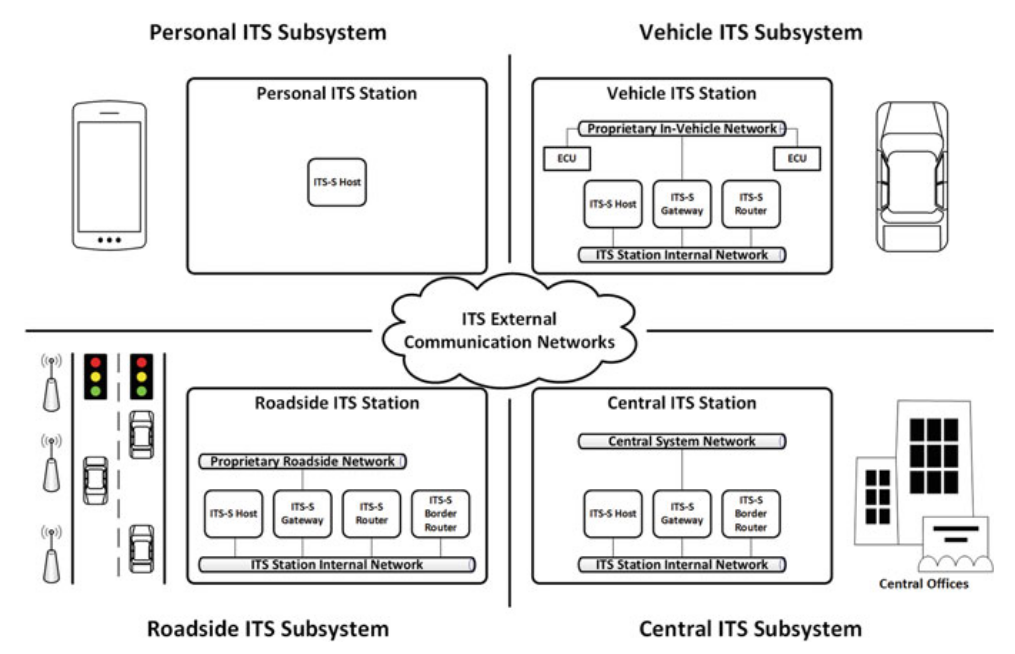
\includegraphics[width=12cm]{Framework/Images/ITSArc.png}.
    \caption{European ITS communication sub-systems}
    \label{cits---s}
\end{figure}
\subsection{Vehicular Communication}
As mentioned above, vehicular communication plays a vital role in ITS to establish cooperativeness and sharing information.  It is implemented using communication technology based on WAVE/IEEE 802.11p \cite{WAVE}. Depending on the Subsystem a vehicle communicates with the modes are divided into three:

\begin{itemize}
    \item \textbf{Vehicle-to-Vehicle (V2V): } In this mode it communicates with another vehicle.
    \item \textbf{Vehicle-to-Roadside Infrastructure (V2R): } In this mode it communicates with the roadside infrastructure.
    \item \textbf{Vehicle-to-Everything (V2X): } In this mode it can communicate with device in the traffic infrastructure.
\end{itemize}

\begin{figure}[h!]
    \centering
    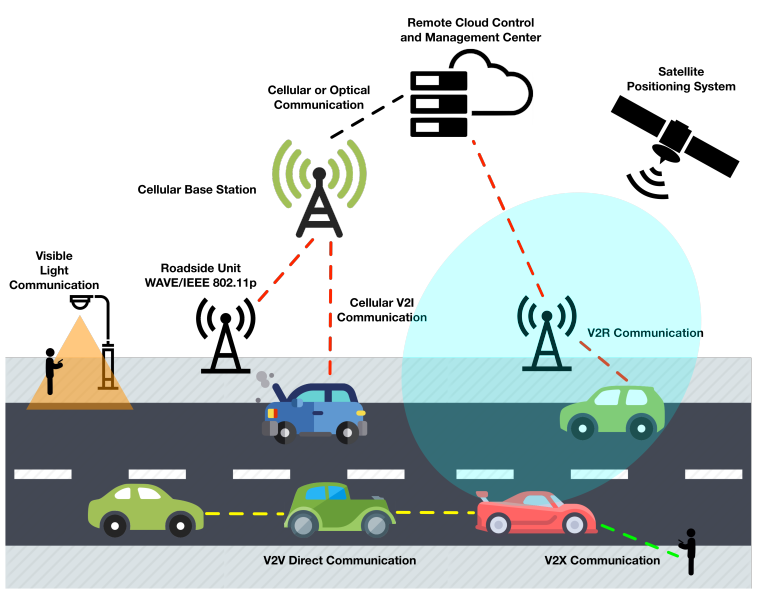
\includegraphics[width=12cm]{Framework/Images/communicationModes.png}.
    \caption{Vehicular Communication Modes \cite{vComs}}
    \label{comsMode}
\end{figure}
\subsection{Cooperative Awareness Message (CAM)}
Cooperative Awareness Message (CAM) \cite{etsiCAM} is a part of the basic cooperative services that are available in all  ITS Stations. CAM is similar to a beacon that is exchanged between an ITS-S and its neighbours to make them aware of their surrounding environment and to enable cooperativness between them. CAM is generated and transmitted periodically but the frequecy is determined by the generating station. 

The content provided by a CAM may vary depending on ITS-S type by all the messages contains the reference position, status and type of the station generating the message. CAM is only transmitted to the stations that are within the communication range of the orginating station and they are not forwarded to other stations once received.
\subsection{Decentralized Environmental Notification Message \\(DENM)}
Decentralized Environmental Notification Message (DENM) \cite{etsiDENM} is a part of basic cooperative service to support the Road Hazard Warning (RHW) application and available in all the ITS stations. DENM is used to notify and warn ITS Stations and users about events that are hazardous to the traffic flow (i.e. vehicle breakdown, accident, lane status, etc..). ITS application triggers and generates DENM upon the occurrence of an event. DENM transmission is repeated and lasts until the triggered event is resolved. A DENM broadcast is terminated once the predefined time limit set by CA service expires or by the ITS application that triggered the DENM.

The DENM contains information about the event that triggered it along with the type and location of the event. DENM are broadcasted through vehicle-to-vehicle (V2V) and vehicle-to-infrastructure communication. Once received, a station forwards the DENM to other stations and only shows the relevant notifications to the driver.

\section{ Current State of the Art in ITS Simulation}
Veins is a popular vehicular network simulation framework researchers use for ITS simulation and evaluation. In this paper \cite{ITSref}, they created an C-ITS applications by extending it to evaluate the application's Quality of Service (QoS). An overview of Viens and its simulation technique is briefly described in the next section before discussing the paper.

\subsection{Veins}
Viens is a simulation framework that performs vehicular communication simulation. It uses OMNET++, discrete-event network simulator and SUMO, discrete-time traffic simulator and binds them using Traffic Control Interface (TraCI) a protocol based on TCP socket. Veins simulate both OMNET++ and SUMO parallelly, and TraCI creates a bidirectional-coupling and make the simulators interact with each other. 

SUMO simulate traffic based on the demand and generates movement trace and sends it to OMNET++. Then, the network simulator updates all the nodes based on the movement trace simulates communication and sends back the simulation result to SUMO.

Viens implemented vehicle and roadside ITS subsystem as network entities to perform vehicular communication. Each entity contains three components and they are extended to create new ITS application, the components are
\begin{itemize}
    \item \textbf{Network Interface Card (NIC): } It implements protocols and stack required vehicular communication
    \item \textbf{Mobility: } It is responsible for the mobility of the network entity, it configures the position based on the movement trace for a vehicle or a static position for RSU 
    \item \textbf{Application: } It implements application, that generates and shares message based traffic information  to perform a basic simulation.
\end{itemize}

\subsubsection{Bidirectionally Coupled Simulation}
Viens extended both the simulators and added a communication model to exchange and buffer commands and messages ( e.g., simulation results, movement trace).  

Since OMNET++ is a discrete-event simulator, it should be triggered to perform the simulation. The framework schedules a trigger at a regular interval to update the node movement and perform the simulation. It follows the same trigger approach for SUMO, as it is a discrete-time simulator the approach suits well. The communication module buffers any messages received by the simulators until the next trigger. 


\begin{figure}[H]
    \centering
    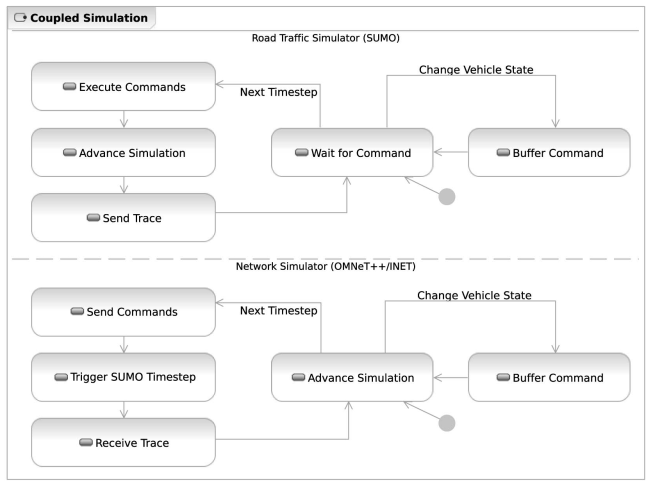
\includegraphics[width=12cm]{Framework/Images/veins1.png}.
    \caption{ Flow Diagram of the simulation \cite{veins}}
    \label{v1}
\end{figure}

\begin{figure}[H]
    \centering
    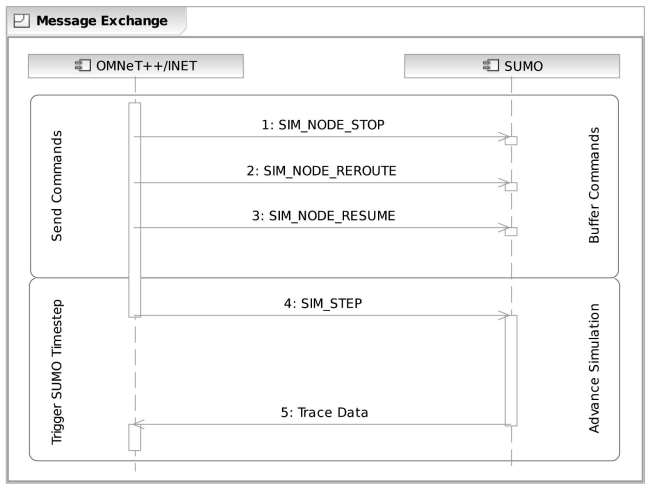
\includegraphics[width=12cm]{Framework/Images/veins2.png}.
    \caption{ Sequence diagram of messages exchanged between simulators \cite{veins}}
    \label{v2}
\end{figure}

At each time step, OMNET++ sends the simulation result as commands and trigger to SUMO, then SUMO performs traffic simulation. After the simulation, SUMO sends the generated movement trace back to OMNET++ and waits for the next trigger. This way OMNET++ updates the position of all the nodes based on the movement trace received from SUMO and performs simulation until the next trigger. During the simulation, OMNET++ makes its nodes interact with inter-vehicle communication and reassign their attributes (e.g., speed, route). In this process, SUMO computes the behaviour of each vehicle in the traffic based on the attributes (e.g., speed, route) of the corresponding nodes. Figures \ref{v1} and \ref{v2} illustrates the entire process.


\subsection{Extending Veins for ITS Application Simulation}
Veins is extended to implement multiple ITS application to evaluate the  QoS of the message broadcasting model. The applications implemented are:
\begin{itemize}
    \item Hazard warning (HW), an event-driven road Safety application
    \item Dynamic speed limit (DSL), a traffic management application
\end{itemize}

First, they create the Traffic Manager Control (TMC) application entity class, it is inherited from BaseWAVEApplLayer class. Then they override the custom application component of Veins RSU with TMC. Now, Veins RSU is customised to send HW and DSL messages. Likewise, the application component of the vehicle entity is overridden with CarApps class. Now, Venis is fully extended and ready for the ITS simulation

\begin{figure}[h!]
    \centering
    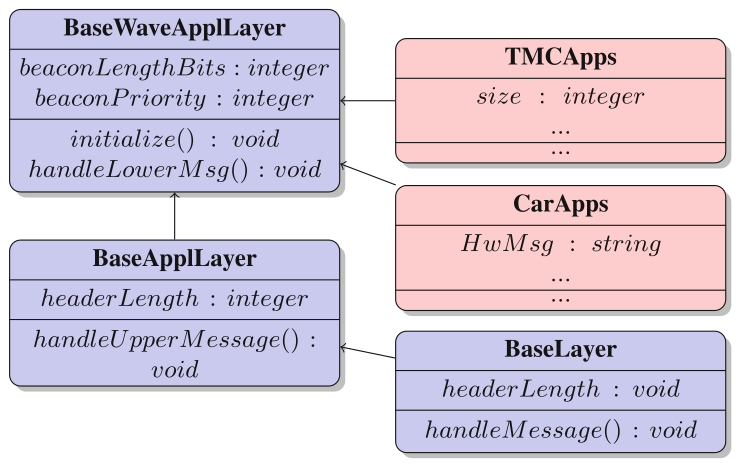
\includegraphics[width=8cm]{Framework/Images/veinsExt.png}.
    \caption{ class of TMC and CarApps  \cite{veins}}
    \label{vExt}
\end{figure}

\section{Tools}
This section discusses the various tools used by the framework to perform the simulation. The framework uses Carla Server as a simulation engine and CarlaViz to visualize the entire simulation in a webpage.
\subsection{CARLA}
\say{CARLA is an open-source autonomous driving simulator} \cite{carla_simulator_2020}. It provides a set of API to perform autonomous driving simulation and build as a tool to help researchers and companies to \say{democratize autonomous driving R&D} \cite{carla_simulator_2020}. It used the Unreal Engine to compute physics and perform simulation and follows the OpenDRIVE standard to design road network and related settings. The simulation performed by the Unreal Engine is controlled by its API provided by Carla in Python and C++. Apart from autonomous driving R&D,  this is a great tool to simulate mobility.

\subsubsection{Architecture}
Carla is built based on a client-server architecture pattern. The server is coupled with the Unreal Engine, and it holds sole responsibility for simulation (i.e., physic computation, sensor and scene rendering are performed). The server is divided into two components based on the elements they control in the simulation. The figure \ref{carc} illustrates the architecture of Carla. 

\begin{itemize}
    \item \textbf{World Server: } This component is responsible for creating the simulation environment. This includes the building, road network, actors (vehicles, sensors and other static properties) etc. It is used to initiates sessions to perform the simulation. Once, initiated it sets the simulation world where actors can be placed.
    \item \textbf{Agent Server: } This component is responsible for the simulating actors. It provides two threads, Control Thread (It receives commands for simulation from a client) and   Measurements Thread (It streams the live sensor data from the simulation).
\end{itemize}

The Carla Server only creates the platform and provides the infrastructure for performing the simulation. The behaviour of all the element is controlled by the Carla Client. A user can gain complete control over an actor, starting from creating it and controlling their behaviour throughout their lifetime. 

\begin{figure}[h!]
    \centering
    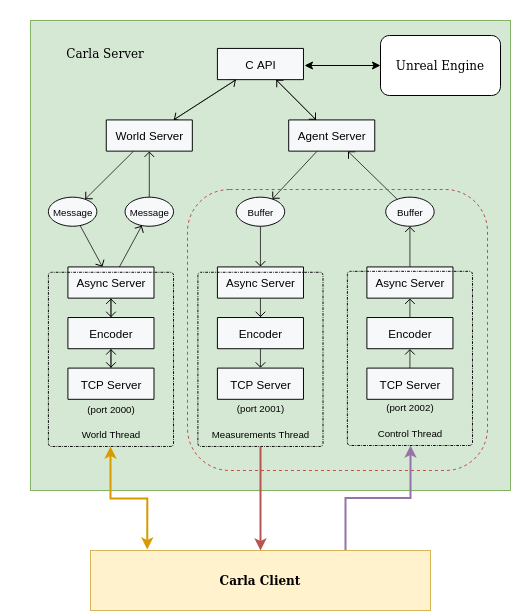
\includegraphics[width=12cm]{Framework/Images/carlaArc.png}.
    \caption{Carla Architecture \cite{carla_simulator_2020}}
    \label{carc}
\end{figure}

\subsubsection{Client-server synchrony}
This section explains about different modes of communication between a client and the server. The server runs in Asynchronous mode by default. In this mode, it simulates as fast as possible without does not wait for any client. On the other hand, in Synchronous mode, the server waits for the client. It proceeds to simulate only if the client gives the signal to do it.

The client can also control the simulation time-step. By default, the server does not follow a fixed time gap, it is called "Variable time-step". The time gap depends on the computation and rendering of physic. The simulation time-step can be fixed by a client. Based on this the server can perform a time-continuous and time-discrete simulation. The figure \ref{carm} shows all the configuration modes provided by Carla.

\begin{figure}[h!]
    \centering
    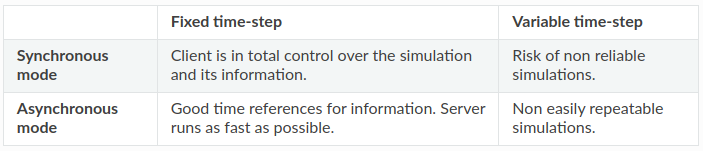
\includegraphics[width=12cm]{Framework/Images/carlaModes.png}.
    \caption{Configuration Modes Provided by Carla \cite{carla_simulator_2020}}
    \label{carm}
\end{figure}

\subsection{CARLAVIZ}
Carlaviz is a visualization plugin developed for Carla to view the simulation environment through a web browser. It streams the world created by the server along with the actors (i.e. Vehicles and pedestrians) living in them and updates their status on the air. Along with this, it streams data from the sensors and visualizes using tables and graphs. Added to this, Carlaviz also allows users to draw texts, points and lines on the visualization. The figure is the sample screenshot of the visualization.

\begin{figure}[h!]
    \centering
    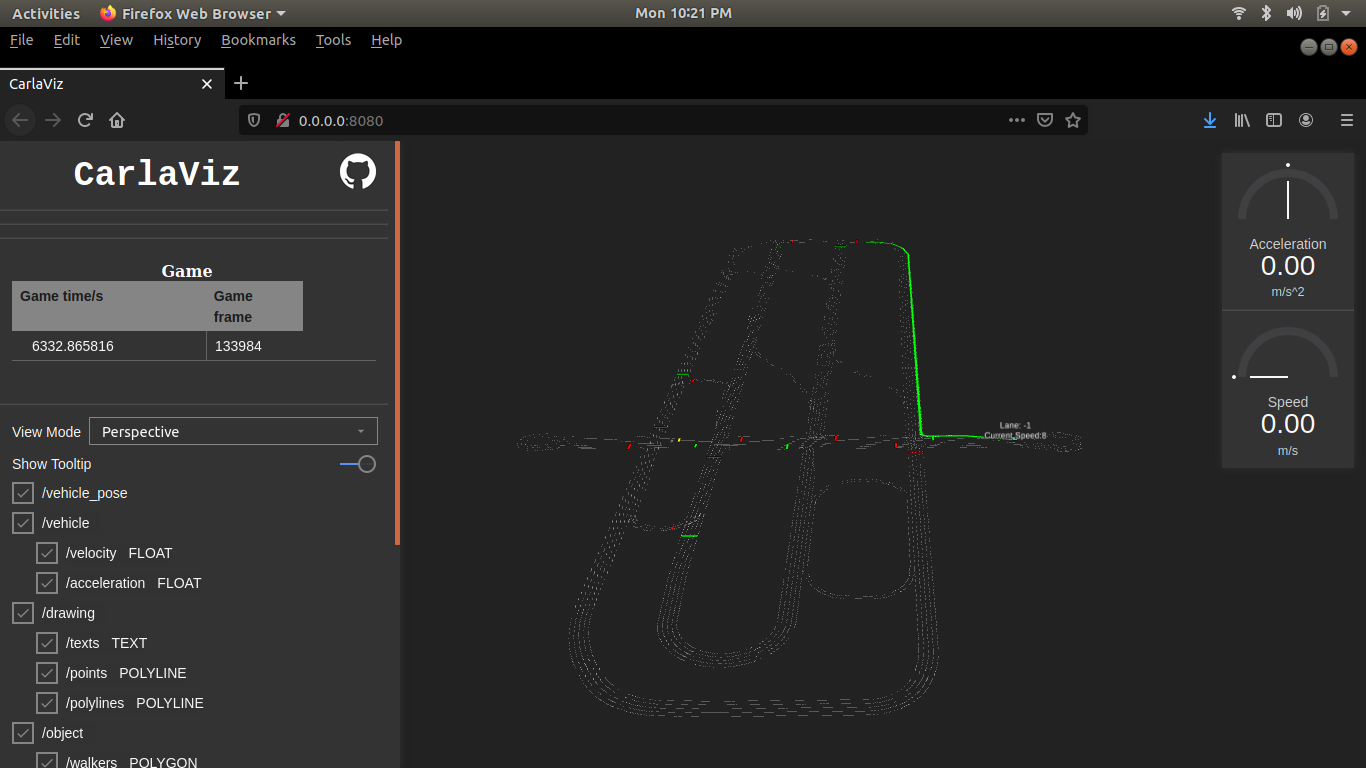
\includegraphics[width=15cm]{Framework/Images/caraVIZ.png}.
    \caption{CarlaVIZ Visualisation Screenshot}
    \label{carm}
\end{figure}
